\section{背景}
电子计算机自诞生以来,经历了快速而显著的发展。在短短的百年时间里,计算机在体积、能耗、计算速度和应用能力等方面都发生了巨大变化。
然而,要充分发挥计算机的潜力,必须使用能够被其解释和执行的指令序列,即程序。
最初,这些程序是通过机器语言编写的,但由于其不直观,极大地限制了计算机的普及。为了解决这一问题,1957年,第一个自动编译器FORTRAN诞生了。
此后,许多性能更高且支持接近自然语言的编译器相继被设计出来,如C/C++编译器GCC,Clang。编译器的出现极大地推动了计算机在现代社会的广泛应用。

\par
为了便于使用计算机,人们首先需要按照特定规则(即程序设计语言,例如C++语言)将待执行的指令以特定顺序编写成源代码。这些源代码随后通过编译器自动翻译(即编译)为一系列机器语言指令(即汇编语言),最后通过链接器各种库文件(链接库),生成可执行程序,并提交给计算机执行。
源代码是程序的初始形式,通常以高级编程语言编写,具有良好的可维护性,并且形式上更加接近自然语言。而汇编语言则是一种机器语言,本质上是由01一一序列映射成的低级程序设计语言,如\autoref{fig:ass}所示,一条汇编语言语句通常由操作码,操作数组成,操作题提供本条指令要执行的操作,而操作数提供数据的来源,\autoref{fig:ass}中展示的汇编语句的作用是 将寄存器rdx和rax中的数据取出来相加,然后把结果放回到rdx寄存器中。
\begin{figure}[H]
    \centering
    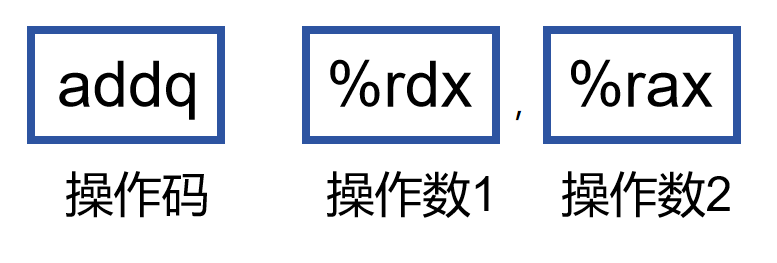
\includegraphics[width=0.8\textwidth]{figures/ass.png}
    \caption{汇编语句的组成}
    \label{fig:ass}
\end{figure}
编译器则是将源代码翻译为机器语言的工具,汇编语言作为机器语言的中间形式,提供了一种更易于理解和操作的方式。编译器的工作流程如\autoref{fig:compiler}所示。编译器会根据源代码构建一个语法树,然后根据语法树的规则转翻译源代码为汇编语言代码。不同版本的编译器在转译时有部分不同的处理方式,例如通过指令调度算法来减少跳转,寄存器换名技术来消除数据冲突。
\begin{figure}[H]
    \centering
    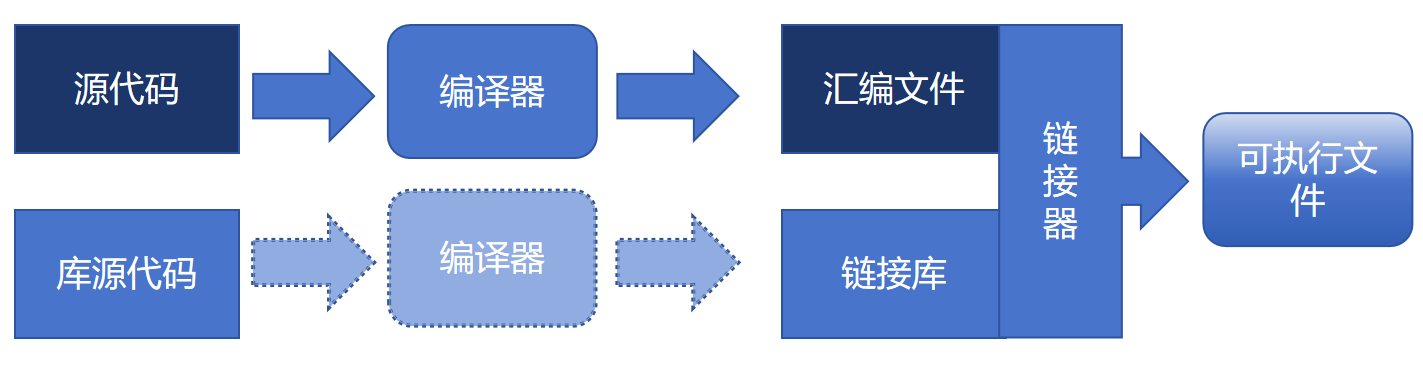
\includegraphics[width=0.8\textwidth]{figures/compiler.png}
    \caption{编译器的工作流程}
    \label{fig:compiler}
\end{figure}
随着编程语言的演变,编译器也在不断更新。例如,GCC(GNU Compiler Collection)已经更新到13.2.0版本。不同版本的编译器在编译同一程序时可能产生不同的编译结果;即使是相同版本的编译器,使用不同的编译选项也会导致编译结果的差异。因此,研究如何利用这些差异来区分编译器的版本具有重要意义。
\par
